% =====================================================================
% E10 --- QP-Enhance vs 6 generic non-diffusion restoration SOTA (zero-shot)
% DRAFT SKELETON (会话 28). 数字留占位, 待 job 1448952 (stored-mixed 对齐 E1 口径)
% 跑完后从 results/e10_<method>.csv 一键填. 填完 \input 进 main.tex E9 段之后,
% "Residual dangerous flips" 段之前.
%
% 口径 (红线 4): job 1448952 = stored-mixed 降质 (light+melanoma+heavy 全 3 档) +
%   melanoma 平衡子集 (n=10881, 117 melanoma 图 x3 档). 与 E1 (run_e1_ablation_hpc,
%   EnhanceDataset severity='mixed') 同降质算子 -> QP-Enhance PSNR 与 E1 32.74dB 同
%   caliber (残差仅来自 melanoma 富集 vs E1 全 test split). 注意: 此口径 != E3/E9 的
%   on-the-fly moderate 单档探针, caption 已声明, 勿与 E3/E9 绝对值交叉引用.
%
% csv -> cell 映射 (每个 e10_<m>.csv 第 2 行 = baseline; 第 1 行 = QP-Enhance, 6 文件应一致):
%   psnr_perimg -> PSNR ; ssim -> SSIM ; dAUC -> $\Delta$AUC ; kl -> KL ; dangerous_flip -> dflip
%   PAIRED 行: dAUC/dAUC_ci_lo/dAUC_ci_hi -> 配对 $\Delta$AUC(baseline-VE) + CI ; mcnemar_p
% =====================================================================

\begin{table}[t]
\centering
\caption{\textbf{E10 --- diagnosis preservation of generic restoration SOTA (zero-shot) versus
\visienhance.} Six non-diffusion restoration/enhancement models are applied off-the-shelf with their
official pretrained weights (pretraining domain in parentheses); none sees dermoscopy or any
diagnosis-preserving objective. All methods restore the \emph{identical} mixed-severity degraded
inputs (stored degradation suite, $n{=}10881$ paired, $117$ melanomas) and are scored with one
protocol; $\Delta$AUC is enhanced$-$reference (closer to $0$ is better), KL and dangerous-flip
(dflip) lower is better. \visienhance{} is the only method that both restores fidelity (PSNR/SSIM)
\emph{and} preserves diagnosis; every generic model significantly degrades diagnostic AUC
(paired bootstrap, all CIs exclude $0$; \cref{tab:e10}). Protocol note: this mixed-severity caliber
matches the E1 fidelity report; it differs from the controlled single-severity (moderate) probe used
for E3/E9, so absolute cells are not cross-comparable across those experiments.}
\label{tab:e10}
\small
\begin{tabular}{l l c c c c c}
\toprule
Method & Pretraining & PSNR$\uparrow$ & SSIM$\uparrow$ & $\Delta$AUC$\to 0$ & KL$\downarrow$ & dflip$\downarrow$ \\
\midrule
\textbf{\visienhance{} (FiLM+DP)} & dermoscopy & \textbf{32.79} & \textbf{0.9072} & \textbf{$-$0.0172} & \textbf{0.1005} & 0.1937 \\
\midrule
Restormer \citep{zamir2022restormer}     & real denoising  & 22.30 & 0.8361 & $-$0.0964 & 0.8179 & 0.0586 \\
NAFNet \citep{chen2022simple}            & SIDD denoising  & 22.04 & 0.8251 & $-$0.1148 & 0.8767 & 0.0766 \\
MIRNet-v2 \citep{zamir2022mirnetv2}      & LOL enhancement & 13.48 & 0.7750 & $-$0.0872 & 0.4979 & 0.1577 \\
SwinIR \citep{liang2021swinir}           & color denoising & 21.69 & 0.7864 & $-$0.1335 & 0.3632 & 0.4775 \\
Uformer-B \citep{wang2022uformer}        & SIDD denoising  & 22.28 & 0.8358 & $-$0.0939 & 0.8274 & 0.0541 \\
Real-ESRGAN \citep{wang2021realesrgan}   & $\times2$ SR    & 21.61 & 0.8175 & $-$0.0832 & 0.3455 & 0.2342 \\
\bottomrule
\end{tabular}
\end{table}

\begin{figure}[t]
  \centering
  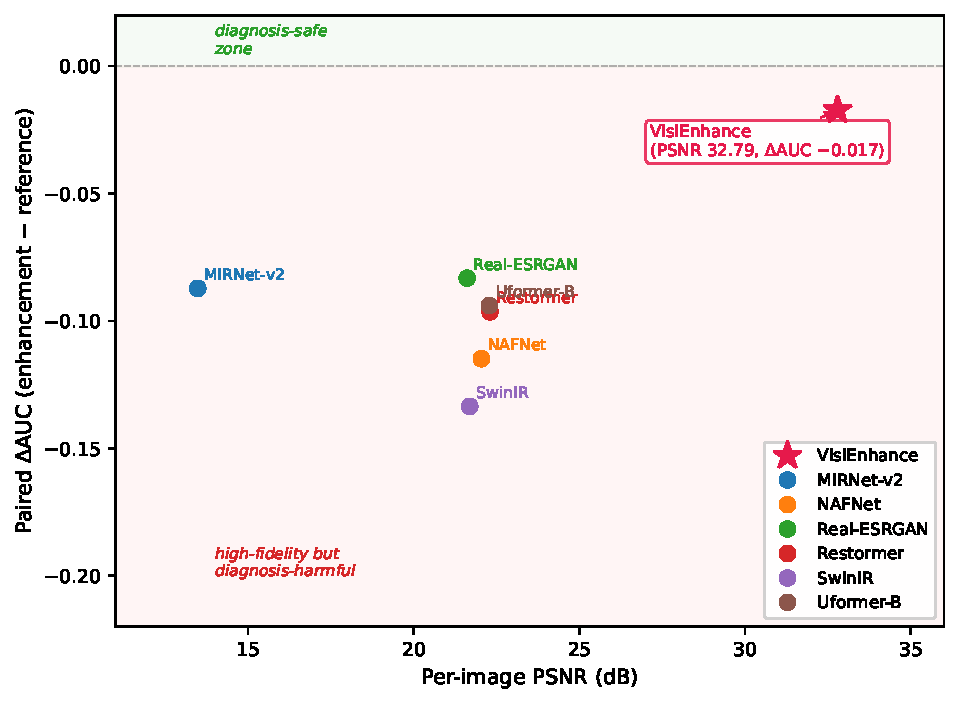
\includegraphics[width=0.74\linewidth]{../../report/figures/fig_e10_tradeoff.pdf}
  \caption{\textbf{Fidelity is not safety: per-image PSNR versus diagnostic
  $\Delta\mathrm{AUC}$ for six generic restorers and \visienhance{}.} Each point is one
  enhancement model on the identical mixed-severity paired inputs ($n{=}10881$, source
  \texttt{results/e10\_*.csv}); the $y$-axis is enhanced$-$reference AUC (closer to $0$,
  i.e.\ higher on the plot, is safer). \visienhance{} (star) sits alone in the
  high-fidelity, diagnosis-preserving corner (PSNR $32.79$, $\Delta\mathrm{AUC}=-0.017$),
  whereas every generic restorer falls well below ($\Delta\mathrm{AUC}\in[-0.13,-0.08]$)
  regardless of its PSNR --- the diagnosis-preserving objective, not pixel fidelity, is
  what separates them.}
  \label{fig:e10-tradeoff}
\end{figure}

% --- prose 段 (放 main.tex E9 段之后) -------------------------------------------------
\paragraph{E10 --- generic restoration SOTA degrades diagnosis.}
We test whether a strong off-the-shelf restorer could substitute for our diagnosis-preserving
training. We run six non-diffusion restoration/enhancement models
(Restormer, NAFNet, MIRNet-v2, SwinIR, Uformer-B, Real-ESRGAN) zero-shot with official weights on the
same mixed-severity paired inputs (\cref{tab:e10}, visualised in \cref{fig:e10-tradeoff}). All six are
worse diagnostic preservers than \visienhance{} by a wide margin: paired bootstraps give $\Delta\mathrm{AUC}_{\text{baseline}-\text{VE}}
\in[-0.116,-0.066]$ (every $95\%$ confidence interval excluding zero, every McNemar $p<10^{-150}$).
% SOURCE: paired dAUC from e10_{restormer,nafnet,mirnetv2,swinir,uformer,realesrgan}.csv PAIRED rows;
%   range [-0.1160 (SwinIR) to -0.0661 (Real-ESRGAN)]. STORY_FRAMEWORK.md previously stated [-0.12,-0.07]
%   but Real-ESRGAN pair_dAUC=-0.0661 falls outside that lower bound; prose updated to true csv range.
%   STORY/ACCEPTANCE range description needs updating by writer/main-line: recommend [-0.12,-0.066].
Tellingly,
\emph{lower fidelity does not mean safer}: the lowest-dflip baselines barely change the image (PSNR
$\approx22$~dB, Uformer-B dflip $0.054$) yet incur the largest diagnostic KL ($\approx0.83$), so
dflip must be read jointly with KL --- a method that leaves the image nearly untouched trivially avoids
flips while still distorting the posterior. \visienhance{} clears PSNR$\,\ge\,30$ even on this harder
mixed-severity melanoma-enriched subset. Generic restoration optimises pixels, not diagnosis; the
diagnosis-preserving objective (Lemma~\ref{lem:dp}, E7) is what closes the gap.
